	\subsection{Wichtige Datenstrukturen, Variablen und Funktionen}\label{sec:ds}
	Auf dem folgenden Bild ist zunächst die Dateistruktur unseres Programmes zu sehen:
	\begin{figure}[h]
	\centering
	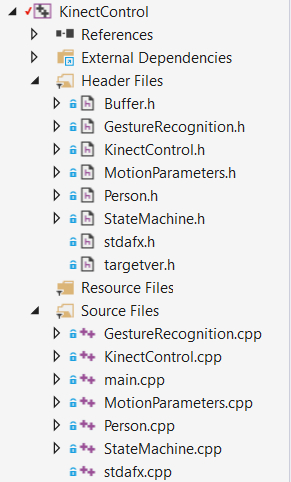
\includegraphics[width=.4\textwidth]{pictures/structure.jpg}
	\caption{Ausschnitt aus dem Solution Explorer der Visual Studio IDE.}
	\end{figure}
	Dabei korrespondieren die Header- mit ihren zugehören .cpp-Dateien zu den wichtigsten Klassen in unserem Programm. Diese sollen nun, sofern dies nicht in den vorangegangen Kapiteln bereits geschehen ist, hinsichtlich ihrer Intention, ihrer Umsetzung und ihrer Verwendung erläutert werden. Die Reihenfolge, in der wir sie vorstellen orientiert sich ihren logischen Abhängigkeiten zueinander.\par\medskip
	\paragraph{KinectControl.} Dies ist unsere Managerklasse, die sowohl als Einstiegspunkt für Aufrufe durch andere Programme dient, als auch zur Gesamtkoordination und Arbeit mit der Kinect Verwendung findet. Wegen ihrer zentralen Funktion, sind alle anderen Header-Dateien in dieser Klasse direkt oder indirekt eingebunden. Insbesondere ist Kinect.h aus dem Kinect-SDK eingebunden, um überhaupt mit der Kinect arbeiten zu können.\par 
	KinectControl stellt eine init-Funktion bereit, die die Datenstrukturen, die für die Kinect-Kommunikation gebraucht werden initialisiert und bereitet diverse Puffer durch Speicherallokation und Füllen mit Default-Einträgen vor. Dazu wird der KinectSensor geholt und \glqq geöffnet\grqq{}, d.\,h. seine Nutzung ermöglicht. Anschließend kann über den KinectSensor auf die BodyFrameSource des Sensors zugegriffen werden, mittels derer man dann durch Öffnen eines Readers den Stream der von der Kinect interpretierten Körperinformationen abgreifen kann. Wir sparen weitere technische Details der Funktion an dieser Stelle aus.\par\smallskip
	Weiterhin spielt die run-Funktion der KinectControl-Klasse eine wichtige Rolle: Sie entspricht dem \glqq Main Loop\grqq{} unseres Programmes. Alle Berechnungen und Aufrufe haben ihren Ursprung in ihrem Rumpf. Im Wesentlichen werden die wichtigen Bestandteile des aktuellen Zustands bzw. bisheriger Berechnungen ausgelesen und mit den von der Kinect erhaltenen neuen Daten abgeglichen oder verrechnet. Einerseits ist unsere Mastererkennung implementiert, zum Anderen findet auch das Puffern der für die Steuerung wichtigen Handpositionen hier statt und schließlich wird von hier aus auch die Zustandsmaschine gesteuert.\par
	\begin{figure}[h]
	\centering
	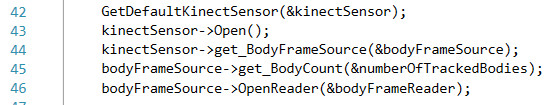
\includegraphics[scale=.5]{pictures/kinectinit.jpg}
	\caption{Ausschnitt aus der init-Funktion.}
	\end{figure}
	%TODO genauer? Quellcodestelle ist grad noch in Arbeit
	\par\medskip
	\paragraph{Buffer.} An dieser Stelle sei auf die Pufferklasse verwiesen. Sie folgt dem bekannten Schema und dient unserem Projekt lediglich als Werkzeug. Auf Details verzichten wir. Es gibt folgende Funktionen:
	\begin{itemize}
	\item Einen Konstruktor, der einen Puffer fester Größe erzeugt; dazu einen Destruktor.
	\item Diverse Zeiger (begin, end und next).
	\item Eine Push-Funktion, sowie eine Funktion zum Leeren des Buffers.
	\item Abfragen auf Gefülltheit und Elemente an gegebenen Positionen.
	\end{itemize}
	Es sei angemekt, dass die Push-Funktion eine Ringpufferfunktionalität implementiert, d.\,h. bei vollem Puffer wird wieder von vorne beginnend überschrieben.\par\medskip
	\paragraph{MotionParameters.} Dies ist eine Hilfsklasse, die eine für uns wichtige Sammlung an Informationen kapselt: Die Bewegungsparameter. Ein MotionParameters-Objekt besteht aus drei Floats, die eine Bewegung in die drei Achsenrichtungen beschreiben, einem Quaternion, der die Rotation enthält und einem \glqq MotionTarget\grqq{} -- einem booleschen Wert, der angibt, ob die Kamera oder ein Objekt manipuliert wird. Darüber hinaus extistieren eine Vielzahl an Gettern und Settern für einzelne oder auch mehrere Klassenvariablen, da es z.\,B.  zweckmäßig ist, die Translationsparameter zusammen setzen zu können (vgl. Zeile 12 in Abb. \ref{fig:motpar}).
	\begin{figure}[h]
	\centering
	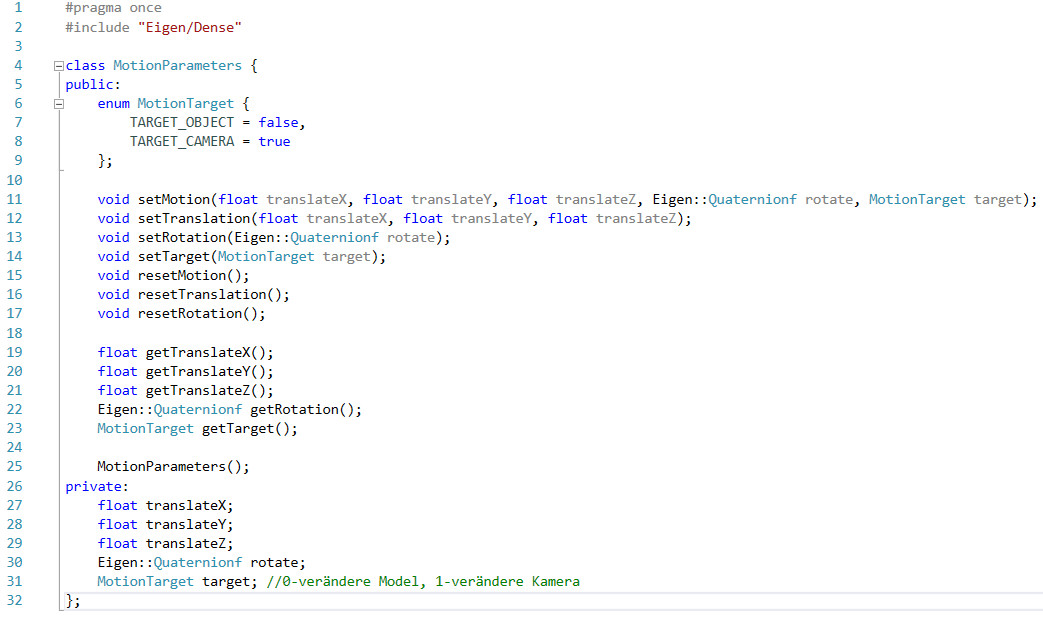
\includegraphics[width=.8\textwidth]{pictures/motionparameters.jpg}
	\caption{Inhalt der Header-Datei MotionParameters.h.}\label{fig:motpar}
	\end{figure}\par\medskip
	\paragraph{Person.} Die Person-Klasse kapselt Informationen, die logisch zu einer von der Kinect erkannten Person gehören. Wir speichern selbstverständlich so gut wie ausschließlich jene Informationen, die wir im Laufe unseres Programmes auch benötigen. Zu einer Person gehören als wohl wichtigstes Element die Gelenkdaten der Kinect -- ein Array von Joints. Ferner werden von diesen Gelenkdaten auch die Orientierungen, gespeichert in einem separaten Array, benötigt. Zentral sind weiter die Puffer für die Positionen der linken und rechten Hand, ein Puffer für die per Geste vorgeführten Rotationen, sowie die HandStates der beiden Hände und eine \glqq ControlHand\grqq{} für die einhändige Objektmanipulation. Dazu verwenden wir eine ID für die Person und verfolgen ihre z-Koordinate. 
	\begin{figure}[h]
	\centering
	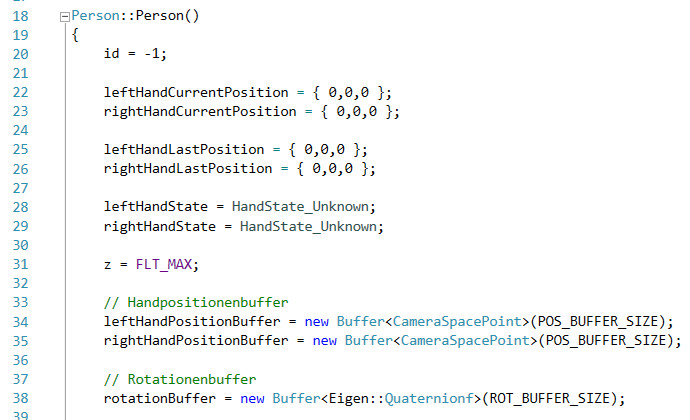
\includegraphics[scale=.5]{pictures/person.jpg}
	\caption{Ausschnitt aus dem Person-Konstruktor mit Initialisierung der wesentlichen Merkmale.}
	\end{figure}\par\medskip
	
	Die weiteren Klassenvariablen dienen verschiedenen Zwecken, unter Anderem stellen sie die Strukturen und Funktionen bereit, die später bei der Mastererkennung dienlich sind. Zentral für die Erkennung ist hierbei die Vermessung der gezeigten Körperproportionen.
	\begin{figure}[h]
	\centering
	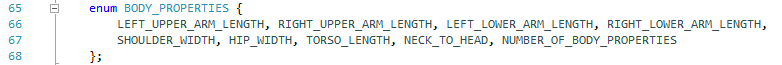
\includegraphics[scale=.7]{pictures/bodyproperties.png}
	\caption{Köperproportionen, die zur Erkennung einer Person gespeichert werden}
	\end{figure}\par\medskip
	
	\paragraph{GestureRecognition.} Hierbei handelt es sich erneut um eine Hilfsklasse. Enthalten sind zunächst die Grundstrukturen für die Arbeit mit unseren selbstdefinierten Gesten. Neben der Definition dieser Gesten selbst als Enumeration ist hier die Struktur \glqq GestureConfidence\grqq{} gespeichert. Ein Behälter, der für unsere verschiedenen Gesten Floats enthält, die angeben werden, wie sicher eine Erkennung der zugehörigen Geste war. Die auf Abb. \ref{fig:gestrechead} ebenfalls zu sehende Enumeration ControlHand ist wieder für die einhändige Objektsteuerung nötig, als Angabe, welche Hand steuert.\par
	\begin{figure}[h]
	\centering
	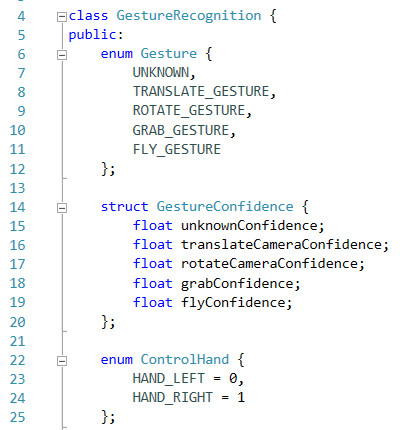
\includegraphics[scale=.4]{pictures/gesturerec.jpg}
	\caption{Ausschnitt aus dem GestureRecognition-Header.}\label{fig:gestrechead}
	\end{figure}	
	Die Hauptfunktion dieser Klasse ist schließlich, neben dem Rahmen der Struktur GestureConfidence, für genau diese Konfidenzen einen Puffer nebst Auswertungsfunktion bereitzustellen, welche schließlich anhand der gepufferten Konfidenzen eine Endkonfidenz pro Geste bestimmt und so letztendlich die vermutlich vorgeführte Geste ermittelt, vergleiche Abb. \ref{fig:evalgestbuf}. Dies ist die Geste mit der höchsten ermittelten Konfidenz.
	\begin{figure}
	\centering
	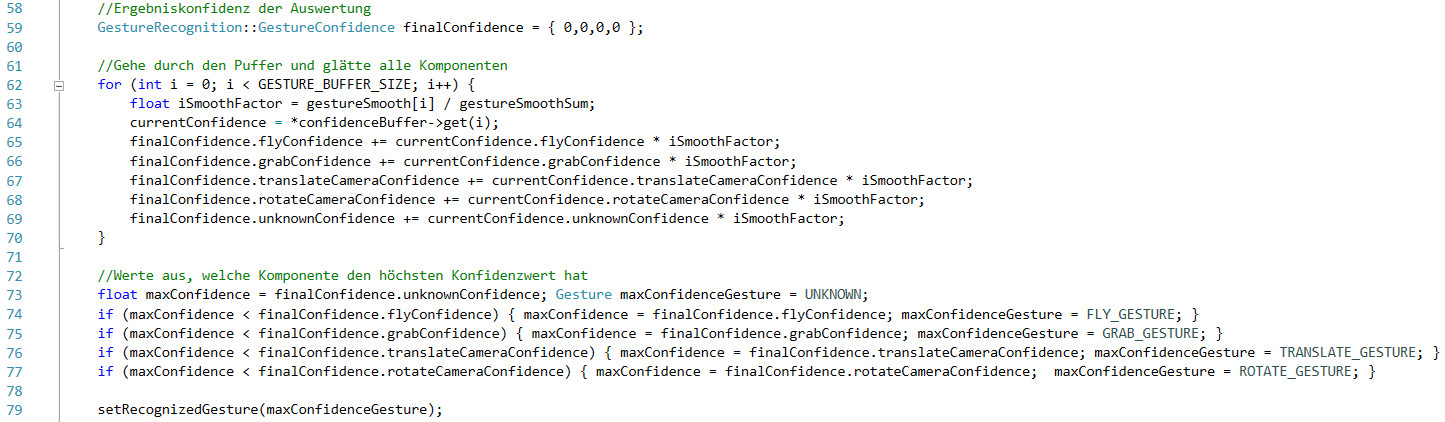
\includegraphics[width=\textwidth]{pictures/gestureeval.jpg}
	\caption{Ausschnitt aus der evaluateGestureBuffer-Funktion.}\label{fig:evalgestbuf}
	\end{figure}
	Die eben genannte \glqq Ermittlung\grqq{} ist dabei einfach eine Glättung der Pufferdaten, Näheres siehe Abschnitt \ref{sec:robustheit}.\par\medskip
	\paragraph{StateMachine.}
	Die Zustandsmaschine ist das Muster, das die Gestensteuerung implementiert. Dem zugrunde liegt die natürliche Abbildung von Steuerungsmodus auf Zustand: Die Zustandsmaschine ist stets gemäß präsentierter Geste in genau einem ihrer Zustände und wertet die gesehenen Daten zu Parametern aus. In der run()-Methode von Kinect-Control wird stets ein Berechnungsschritt, d.\,h. Berechnungen und Zustandswechsel, der State Machine durchgeführt.\par 
	Aus datenstruktureller Sicht ist das State-Struct zentral, das die bereits konzeptuell bekannten Zustände IDLE, CAMERA\_TRANSLATE, CAMERA\_ROTATE, OBJECT\_MANIPULATE und FLY definiert. Wichtige Klassenvariablen sind der aktuelle Zustand \glqq{}state\grqq{}, die eingespeicherte Person \glqq{}master\grqq{}, sowie eine GestureRecognition-Instanz für die Gestenerkennung und die aktuellen berechneten Rückgabeparameter \glqq{}motionParameters\grqq{}. Darüber hinaus enthält sie zahlreiche Konstanten, die als Gewichte, Constraints oder empirisch ermittelte Verstärkungs- bzw. Abschwäschungsfaktoren Verwendung finden.\par 
	Für einen Arbeitsschritt der StateMachine sind die Funktionen bufferGestureConfidence(), compute() und switchState() ausschlaggebend. Diese Funktionen werden in genau dieser Reihenfolge im Main-Loop von KinectControl aufgerufen. In bufferGestureConfidence() wird aus den Kinectdaten unter Prüfung diverser Constraints eine Fuzzy-Geste in Form eines Konfidenztupels bestimmt und gepuffert. Dieser Puffer wird anschließend direkt ausgewertet und liefert die erkannte Geste, die in recognizedGesture gespeichert wird. Die compute()-Funktion errechnet daraufhin je nach aktuellem Zustand aus den gesehenen Skelettdaten und HandStates entsprechend vorangegangener Erklärungen die Bewegungsparameter und legt sie gebündelt in motionParameters ab. Schließlich entscheidet switchState() anhand der recognizedGesture über den Folgezustand und nullt gegebenenfalls die motionParameters der StateMachine.\par 
	\begin{figure}[h]
	\centering
	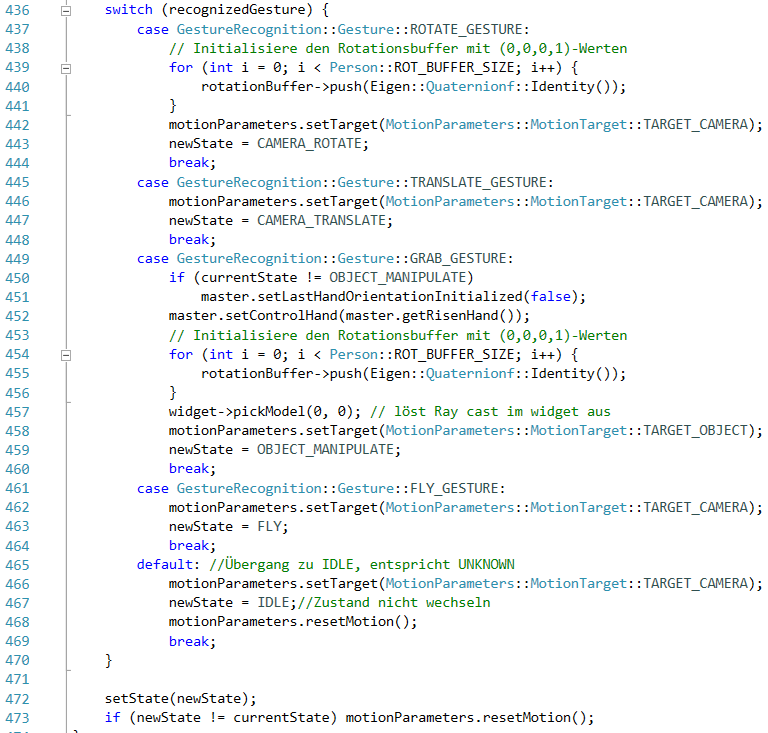
\includegraphics[width=.9\textwidth]{pictures/switchstate.png}
	\caption{Ausschnitt aus der switchState-Funktion.\\Anmerkung: Die pickModel-Funktion in Zeile 457 nutzt eine Stubfunktion, die in einer möglichen Erweiterung der Software zum Object Picking verwendet werden kann.}\label{fig:switchstate}
	\end{figure}
	Das als Erweiterung der Aufgabenstellung eingeführte Eventsystem liegt aufgrund der Klassenhierarchie ebenfalls in der StateMachine-Klasse.